% Source: fixed Guangdong candidate PDF, source-relative page 1, Q4.
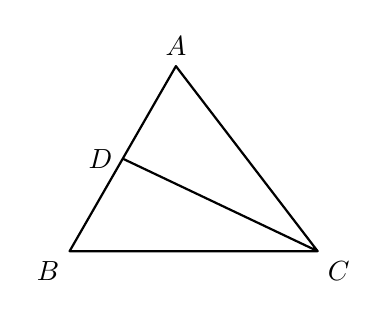
\begin{tikzpicture}[line cap=round,line join=round,thick]
  \coordinate (A) at (1.35,2.35);
  \coordinate (B) at (0,0);
  \coordinate (C) at (3.15,0);
  \coordinate (D) at (0.675,1.175);
  \draw (A)--(B)--(C)--cycle (D)--(C);
  \node[above] at (A) {$A$};
  \node[below left] at (B) {$B$};
  \node[below right] at (C) {$C$};
  \node[left] at (D) {$D$};
\end{tikzpicture}
